% Chapter 6 is usually termed 'Evaluation' or 'Validation'. How did you test it? In which environment? How
% does it scale? Measurements, tests, screenshots. This chapter will have a volume of 10-15 percent of your
% thesis.
% In this chapter the implementation of Component X is evaluated. An example instance was
% created for every service. The following chapter validates the component implemented in
% the previous chapter against the requirements.
% Put some screenshots in this section! Map the requirements with your proposed solution.
% Compare it with related work. Why is your solution better than a concurrent approach from
% another organization?
% - compare the following approaches:
% suite.st
% http://www.eurofins-digitaltesting.com/test-tools/testwizard-automation-suite/

\chapter{Evaluation\label{cha:chapter6}}

Looking back to chapter \ref{cha:chapter3} describing the requirements of the final product we will
evaluate the result and the usability of it in this chapter. The goal was to create a development
and testing environment for HbbTV applications that is comparable with the state of the art of
modern web development. Building web applications for the big screen turned out to be very cumbersome
since there are no tools that help the developer to understand what is going on on the TV. Common
workarounds are self build logging overlays on the developed application which might give information
about certain variable states but don't disclose the insides of the app at all. The DevTools Backend
component is the first tool that allows HbbTV developer to actually inspect a wide variety of aspects
of an HbbTV application.

\begin{figure}[htb]
  \centering
  \hspace*{-0.7cm}
  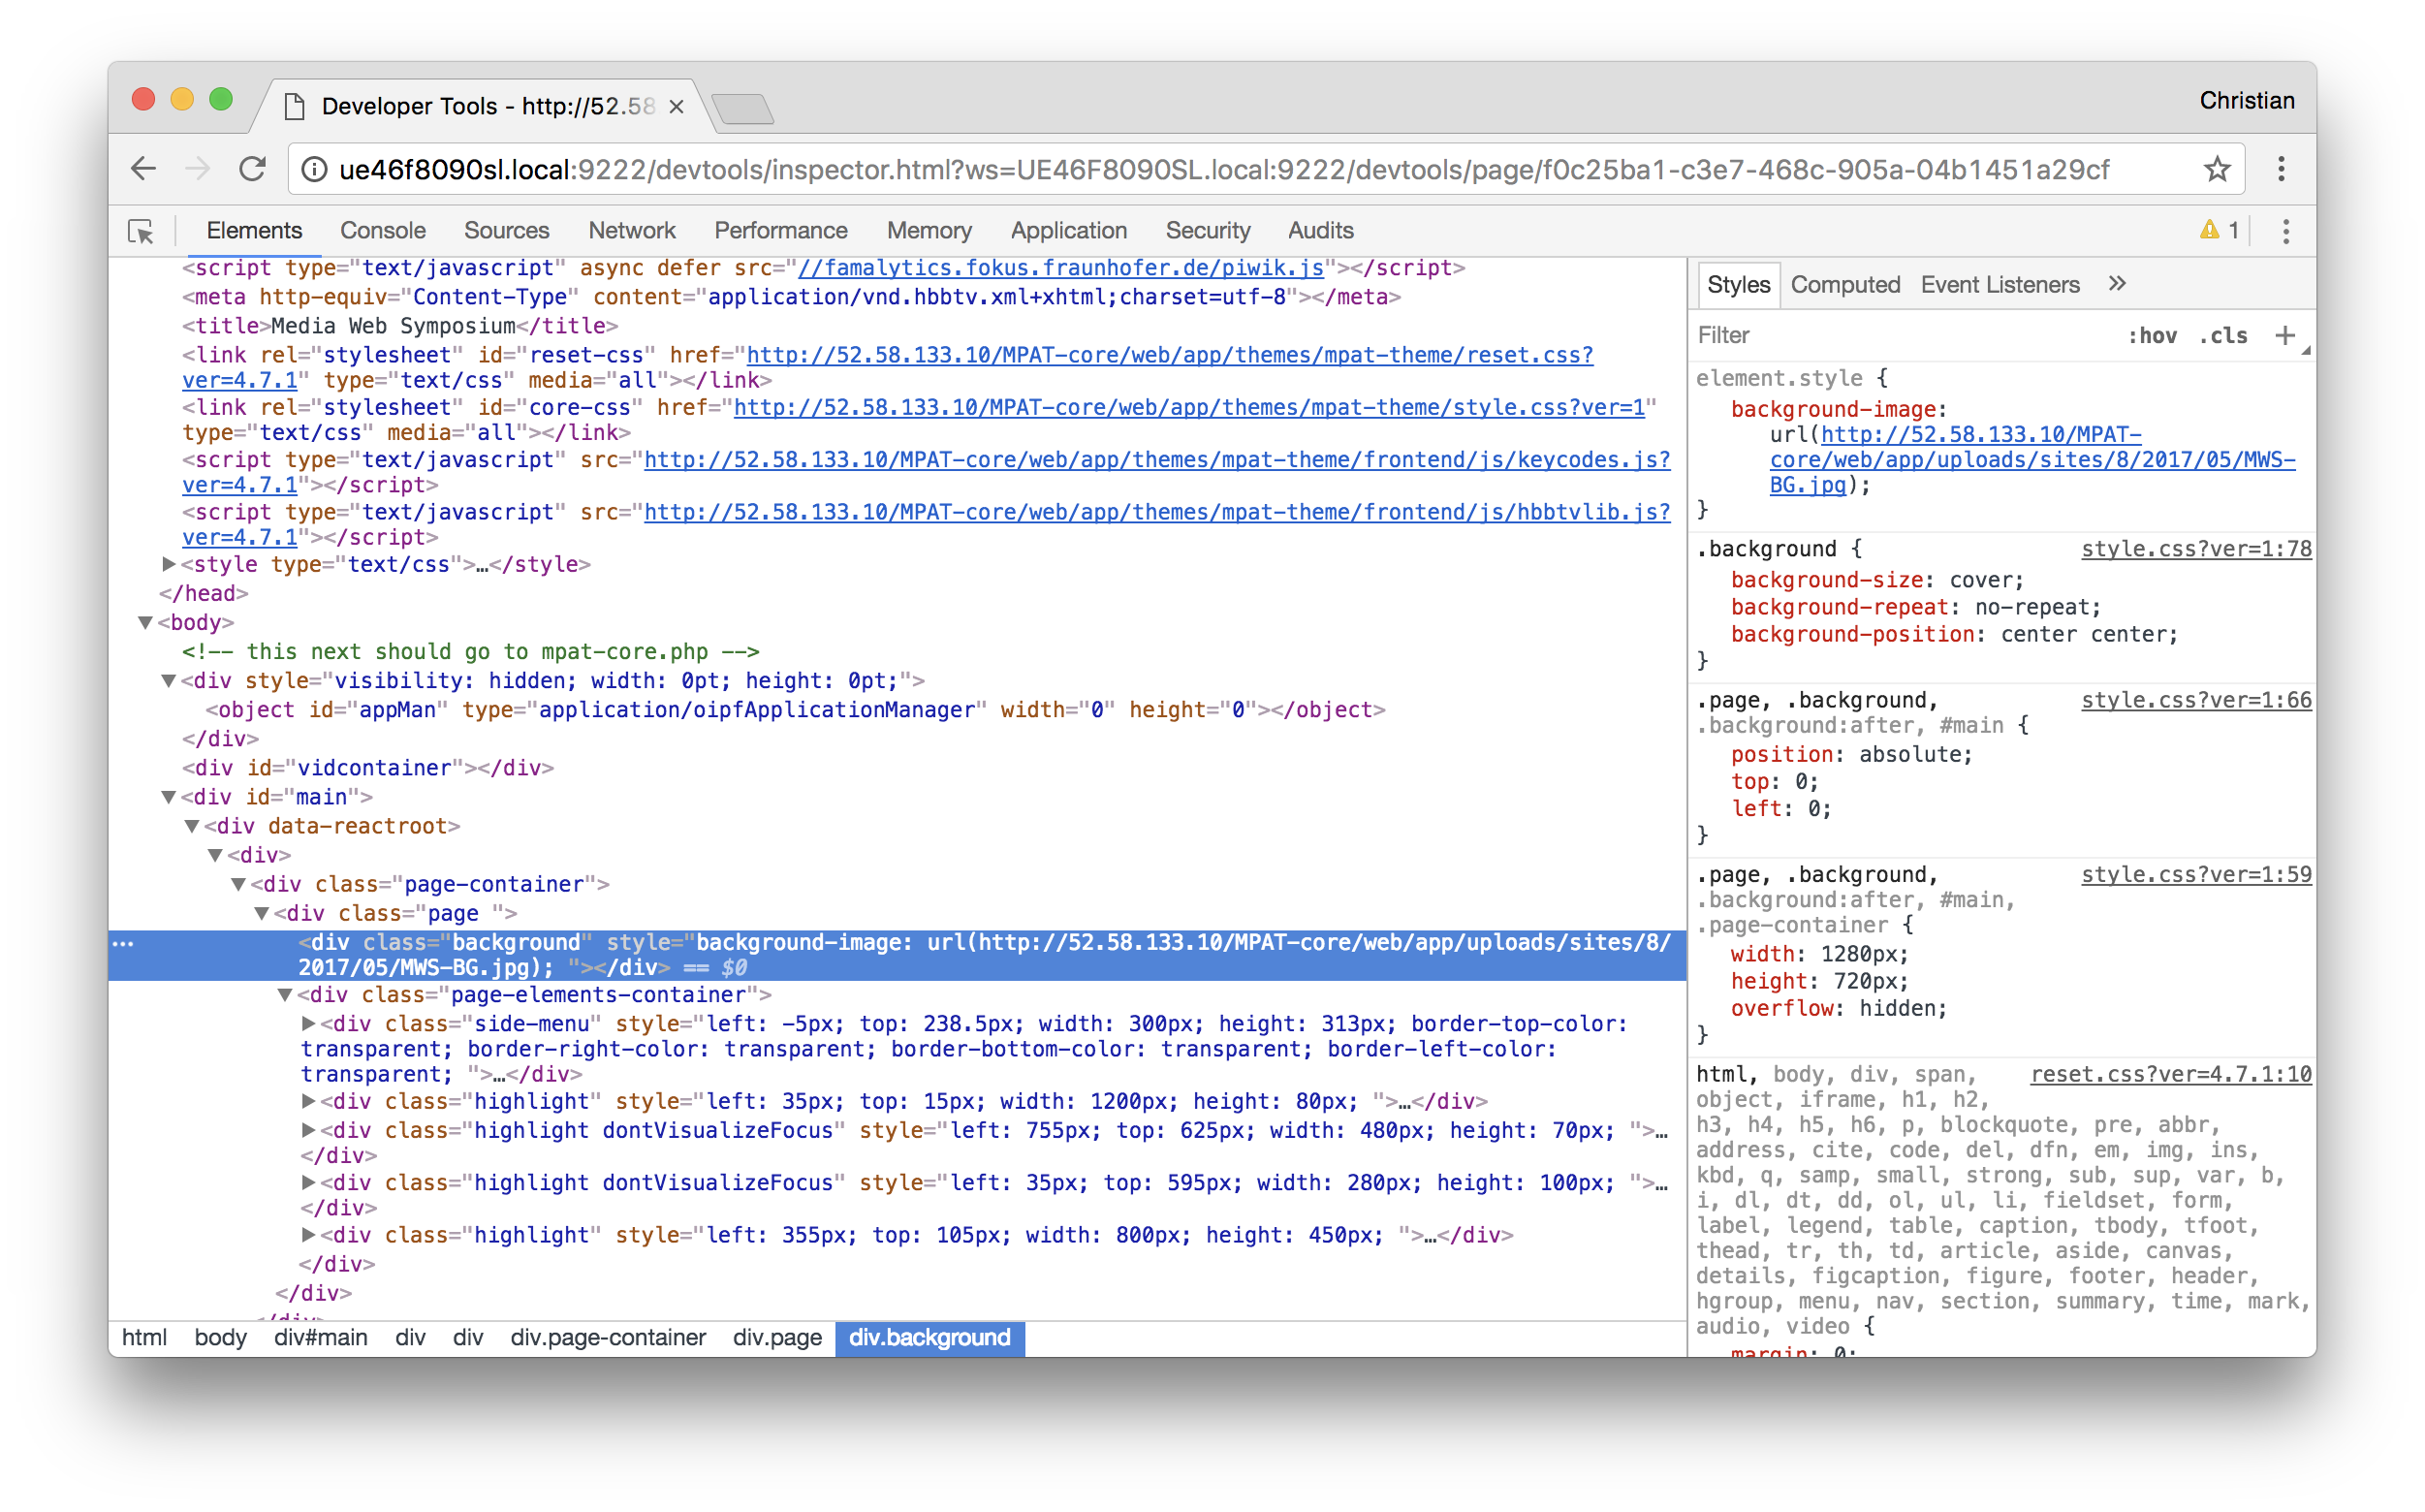
\includegraphics[width=16cm]{elementsPanel.png}\\
  \caption{Inspecting the DOM tree of an HbbTV Application using the DevTools application}\label{fig:elementsPanel}
\end{figure}

It not only allows to look into the DOM tree of the app but also modify elements and their CSS
properties. Developer have now the opportunity to build the app directly on the TV instead of
having to implement it on a browser first to then test it on a real Smart TV. Instead building
a custom logging mechanism it automatically captures all logs from the page as well as JavaScript
errors being thrown. In addition to that the \textit{Console} tab of the DevTools application
allows to execute any random JavaScript code within the context of the HbbTV page. With that it
can inspect variables of your application during runtime. It can be used by the developer to see
which JavaScript APIs are available in the browser environment of a specific target device.

\begin{figure}[htb]
  \centering
  \hspace*{-0.7cm}
  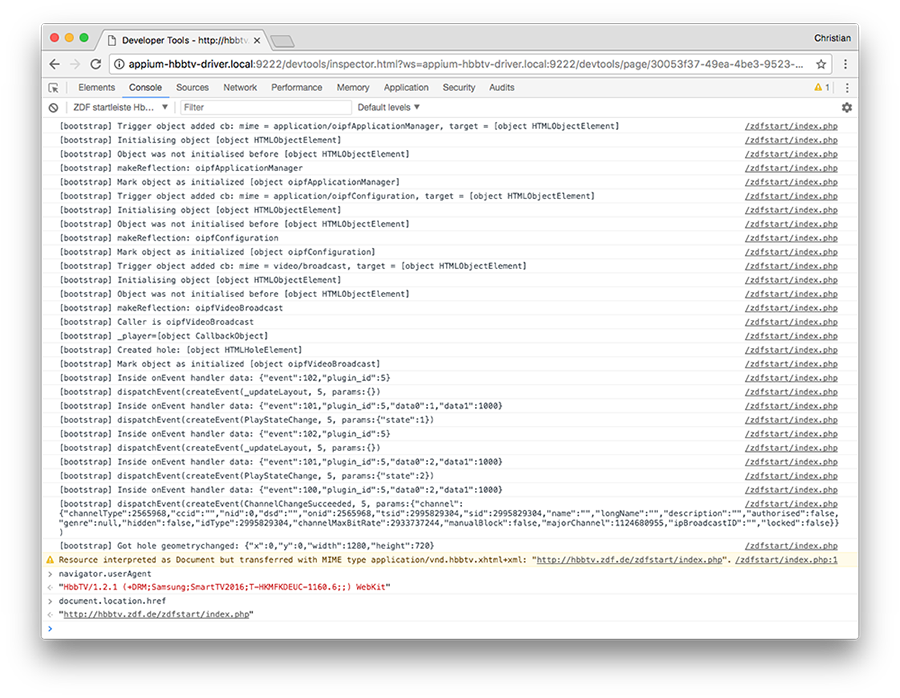
\includegraphics[width=16cm]{consolePanel.png}\\
  \caption{Debugging the ZDF HbbTV application with the Console tab}\label{fig:consolePanel}
\end{figure}

In addition to that since the TV is running all its network traffic through the proxy on the Raspberry Pi
it automatically collects all network data in a way that it can be displayed in the DevTools application as well.
It enables developers using this tool to not only see if all network requests have been resolved successfully
on their own app but also on any arbitrary HbbTV applications that are published. This gives developers and
researchers the chance to look into the loading behavior of an app to reveal information on when certain data
is loaded and if the app is tracking the viewer behavior in any way. Like in the browser the DevTools application
as seen in figure \ref{fig:networkPanel} it shows not only a list of all network requests that have been made by the
app but also their content.

\begin{figure}[htb]
  \centering
  \hspace*{-0.7cm}
  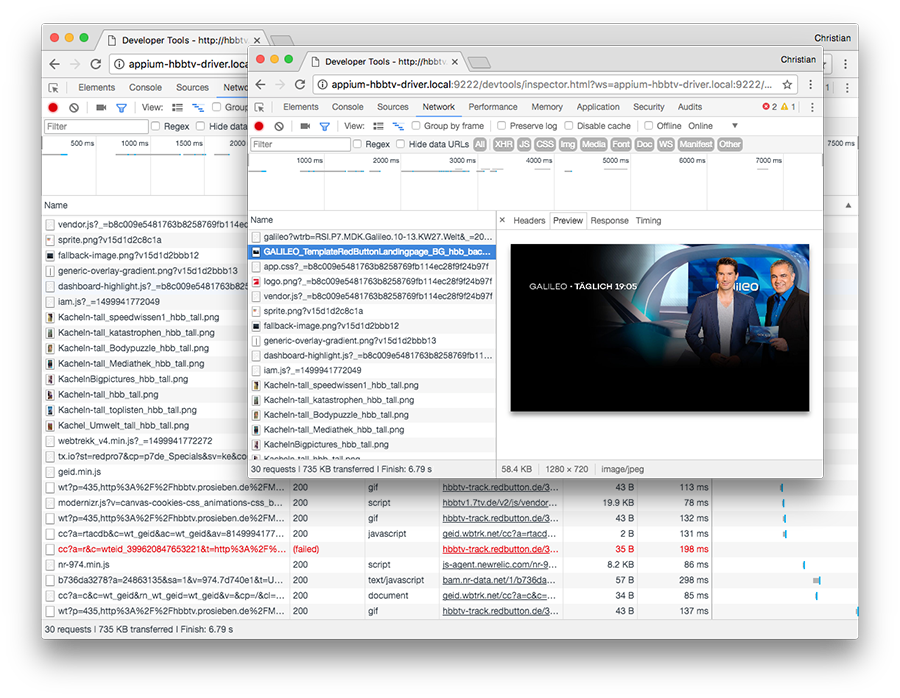
\includegraphics[width=16cm]{networkPanel.png}\\
  \caption{Network requests being made by the Pro7 HbbTV application}\label{fig:networkPanel}
\end{figure}

Sniffing through the requests shows that many small data packages that are covered as 1px gif images are
sending user information to services like INFOnline\footnote{See request details in Annex section under
listing \ref{ioam}} or a New Relic aggregator\footnote{See Annex section under listing \ref{newrelic}} containing
data on the viewer origin, his device, its model name and other device metrics. Another interestung artifact
of data that can be observed when switching aroung pages on the Pro7 HbbTV app. Everytime a new page is
opened a request is send to \url{hbbtv-track.redbutton.de} that tracks the movement of the viewer\footnote{Also
shown in Annex section listing \ref{sniffing}}. After the page has fully loaded you can see at the bottom of the
page that the main page took about 7 seconds to fully and it downloaded 735 KB in 30 requests. This can be used
to leverage interesting metrics of the performance of the HbbTV application.

Not only on the debugging side fulfills this tool all requirements that were stated before also its testing
features raise above everything that has been done in the HbbTV industry before. Until now \textit{''most TV
device browsers don’t support WebDriver''}\cite{sengo}\footnote{The tool that is statet as HbbTV testing solution
that supports Selenium doesn't exist anymore. There are no references on the internet other than this presentation.}
but with the Appium HbbTV Driver developer can for the first time setup a grid of Smart TVs to run WebDriver
tests on them. Since it is based on the WebDriver protocol which is the industry standard for automated desktop
and mobile testing there are already hundreds of libraries available that can be used to write these automated tests.
These libraries are available in all programming languages and flavors and already known by many developers that
have experience with automated tests. As shown in listing \ref{wdioExample} an automation script can be written
in couple lines of code. These tests are fairly simple to write even for non developers. There are solutions like
Cucumber\footnote{\url{https://cucumber.io/}} that allow to abstract away the coding part of these tests by writing
feature files with acceptence sentences which are translated in actual code. This makes writing e2e tests accessible
for everyone.

\section{Comparison To Other Testing Solutions\label{sec:businessmodel}}



\section{Features and Offerings\label{sec:features}}

- Explain provided features

\section{Solution Evaluation\label{sec:usab}}

- Compare solutions
- For which group of people is which solution the better choice

\section{Comparison of writing automated tests for web/mobile vs TV\label{sec:diffInWritingTests}}

- Compare Inpute devices
- JS and environement feature set


- Therefor the tool has to be based on existing standards around automated testing and development
